\begin{center}
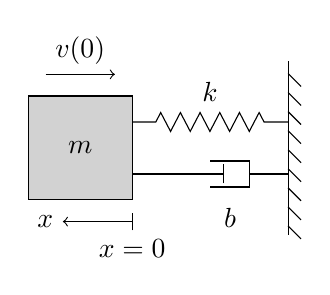
\begin{tikzpicture}[
    scale=1.1,
    spring/.style={decorate, decoration={zigzag, pre length=0.3cm, post length=0.3cm, segment length=0.25cm, amplitude=0.12cm}},
]
  % ---- object (mass) ----
  \fill[gray!35] (0,0.4) rectangle (1.2,1.6);
  \draw (0,0.4) rectangle (1.2,1.6);
  \node at (0.6,1.0) {$m$};

  % ---- buffer: spring (top) and damper (bottom), in parallel ----
  \draw[spring] (1.2,1.3) -- (3.0,1.3);
  \node[above=4pt] at (2.1,1.3) {$k$};
  % damper: piston plate inside an open cup fixed to the wall
  \draw (1.2,0.7) -- (2.25,0.7);
  \draw (2.25,0.59) -- (2.25,0.81);
  \draw (2.1,0.55) -- (2.55,0.55) -- (2.55,0.85) -- (2.1,0.85);
  \draw (2.55,0.7) -- (3.0,0.7);
  \node[below=4pt] at (2.33,0.55) {$b$};

  % ---- wall ----
  \draw (3.0,0) -- (3.0,2.0);
  \foreach \i in {0,...,8} { \draw (3.0,0.1+0.22*\i) -- (3.15,-0.05+0.22*\i); }

  % ---- initial velocity (toward the wall) ----
  \draw[->] (0.2,1.85) -- (1.0,1.85) node[midway,above] {$v(0)$};

  % ---- x axis: x = 0 at the start of the crash, positive away from the wall ----
  \draw (1.2,0.05) -- (1.2,0.25);
  \node[below] at (1.2,0.05) {$x=0$};
  \draw[->] (1.2,0.15) -- (0.4,0.15) node[left] {$x$};
\end{tikzpicture}
\end{center}
